\subsection{Tiling}

\frame{
  \frametitle{Representing Collision Strings}

  \begin{itemize}
    \item Reflect squares about each side to create a tiling
    \item Solutions become lines in the plane
    \item Intersections become places where collisions occur
  \end{itemize}
}

\frame{
  \frametitle{Representing Collision Strings}

  \begin{example}
    Tiling of $\vec{x}_0 = (0, 0.5)$ and $\vec{v} = (0.25, 0.25)$.
  \end{example}

  \begin{columns}
    \begin{column}{0.45\textwidth}
      \begin{figure}
        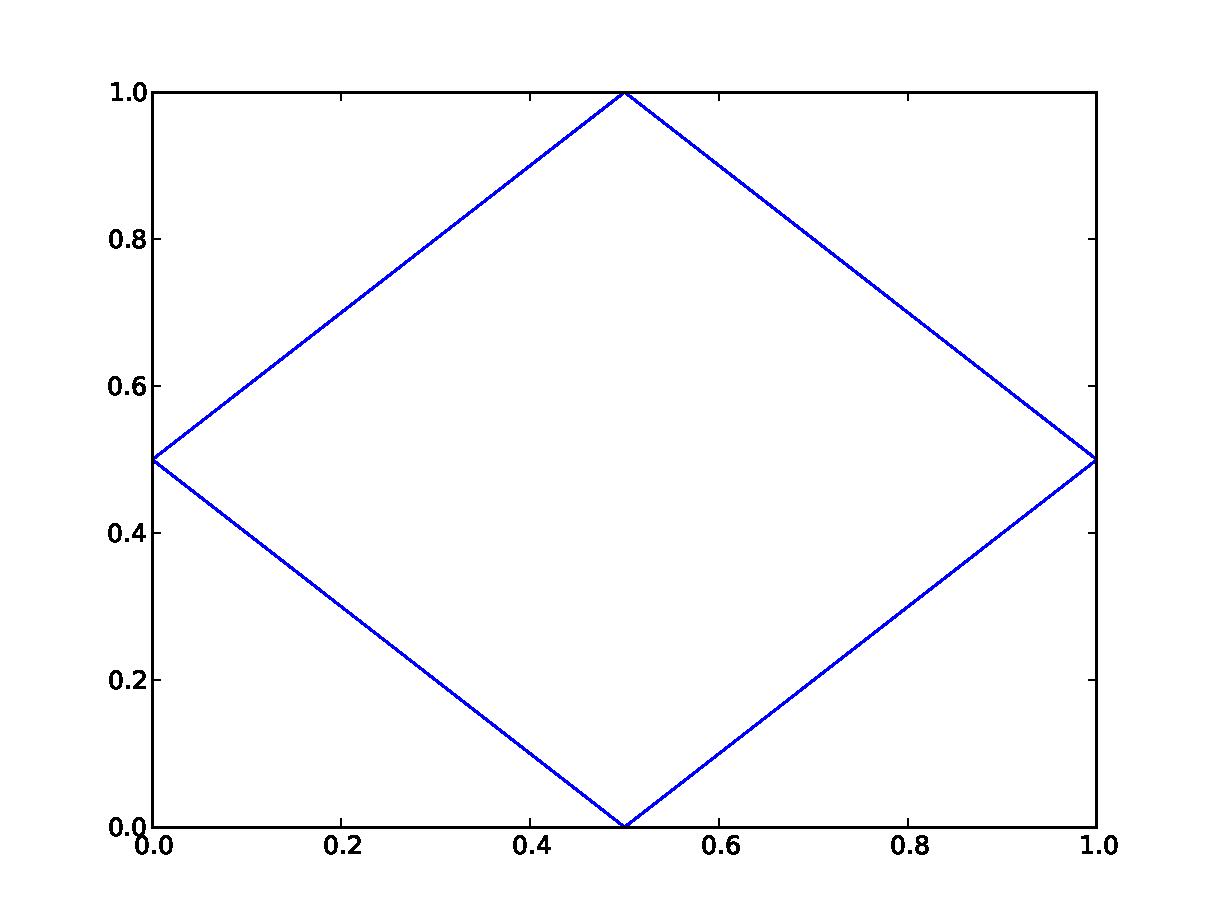
\includegraphics[width=2.1in]{abab.pdf}
      \end{figure}
    \end{column}
    \begin{column}{0.45\textwidth}
      \begin{figure}
        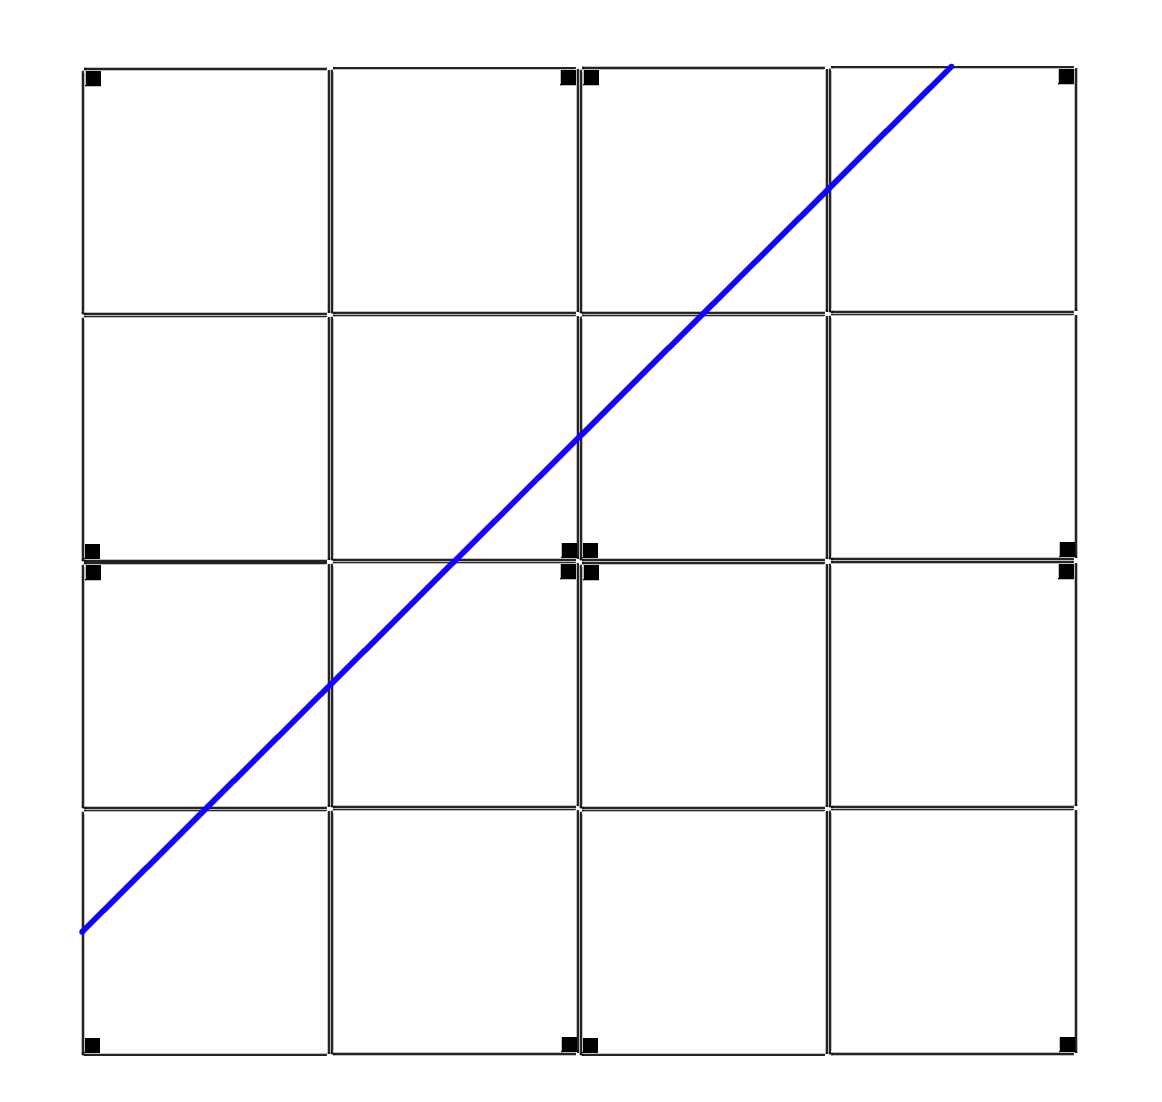
\includegraphics[width=1.7in]{tiling.png}
      \end{figure}
    \end{column}
  \end{columns}
}

\frame{
  \frametitle{Representing Collision Strings}

  \begin{example}
    Tiling of $\vec{x}_0 = (0, 0.5)$ and $\vec{v} = (0.25, 0.25)$.
  \end{example}

  \begin{columns}
    \begin{column}{0.45\textwidth}
      \begin{figure}
        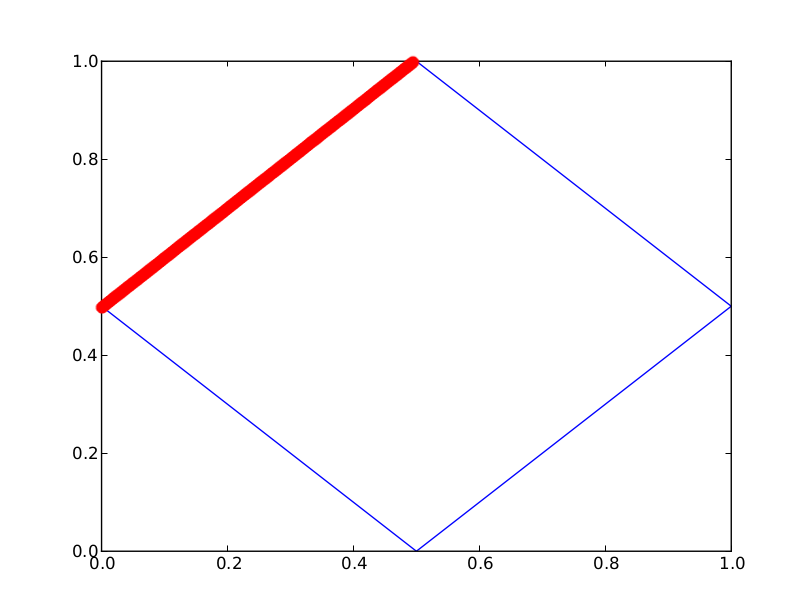
\includegraphics[width=2.1in]{tiling_real_step_1.png}
      \end{figure}
    \end{column}
    \begin{column}{0.45\textwidth}
      \begin{figure}
        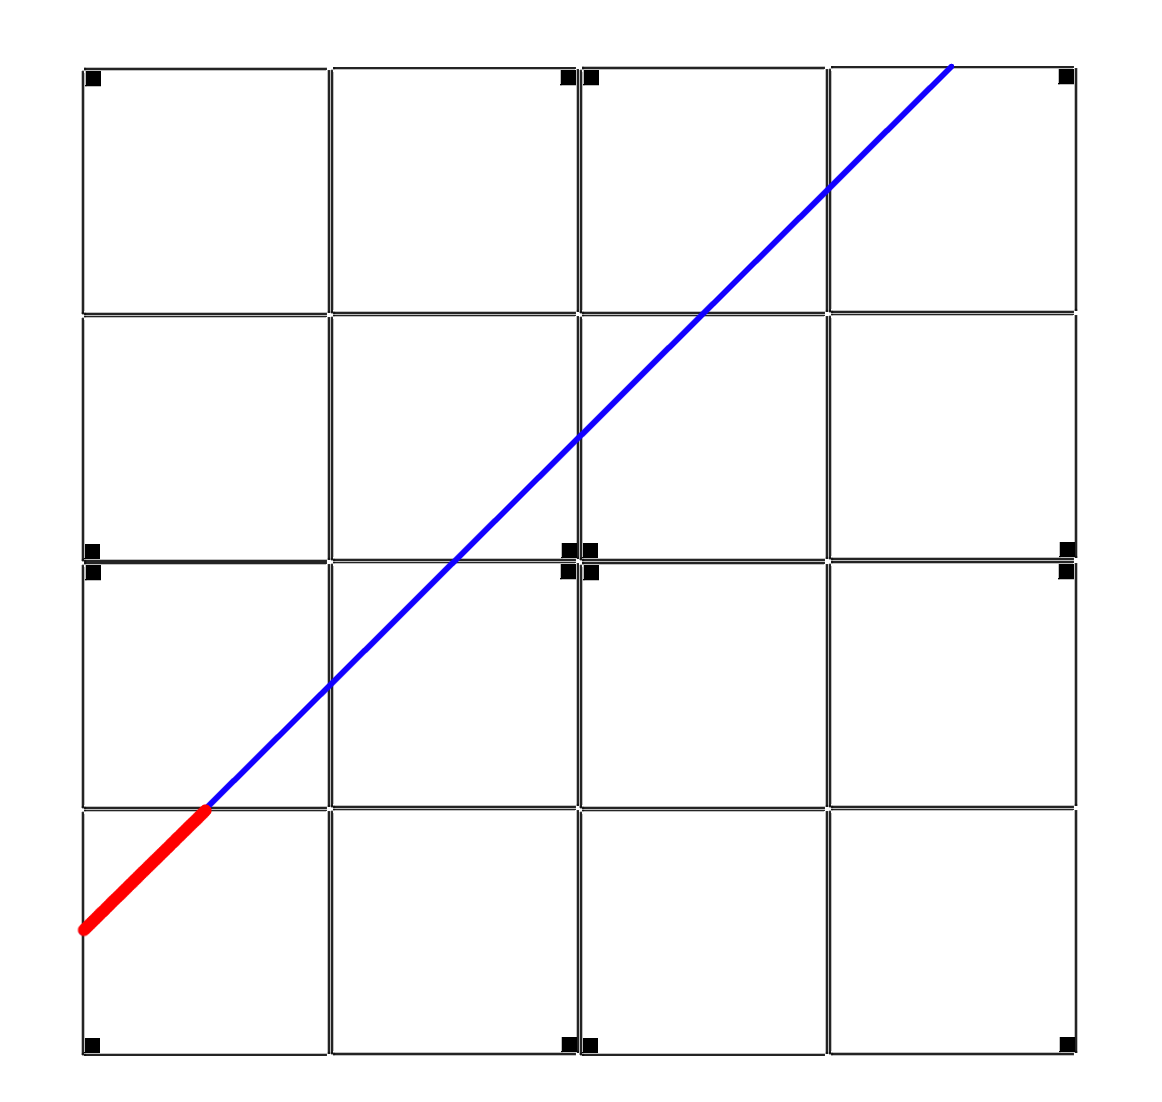
\includegraphics[width=1.7in]{tiling_tiled_step_1.png}
      \end{figure}
    \end{column}
  \end{columns}
}

\frame{
  \frametitle{Representing Collision Strings}

  \begin{example}
    Tiling of $\vec{x}_0 = (0, 0.5)$ and $\vec{v} = (0.25, 0.25)$.
  \end{example}

  \begin{columns}
    \begin{column}{0.45\textwidth}
      \begin{figure}
        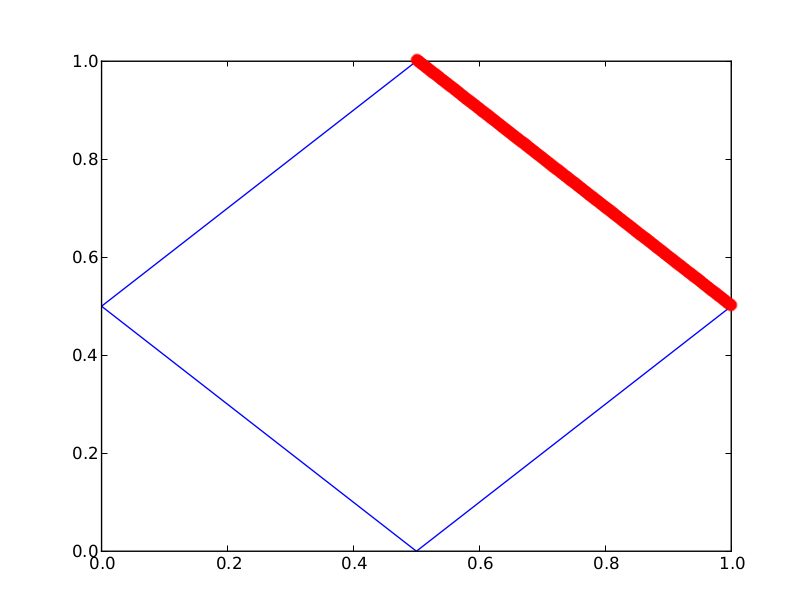
\includegraphics[width=2.1in]{tiling_real_step_2.png}
      \end{figure}
    \end{column}
    \begin{column}{0.45\textwidth}
      \begin{figure}
        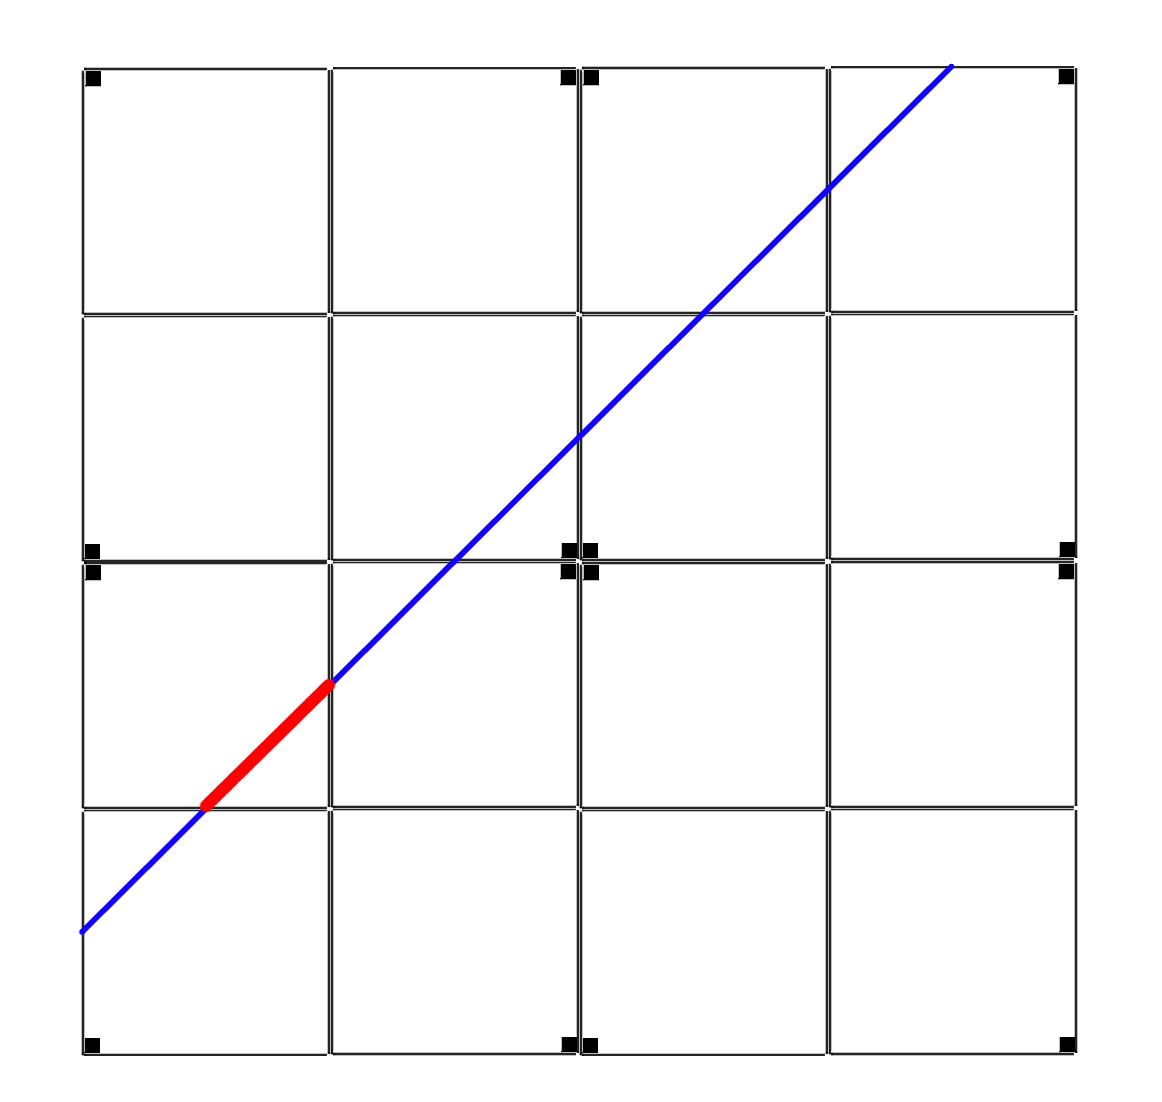
\includegraphics[width=1.7in]{tiling_tiled_step_2.png}
      \end{figure}
    \end{column}
  \end{columns}
}

\frame{
  \frametitle{Representing Collision Strings}

  \begin{example}
    Tiling of $\vec{x}_0 = (0, 0.5)$ and $\vec{v} = (0.25, 0.25)$.
  \end{example}

  \begin{columns}
    \begin{column}{0.45\textwidth}
      \begin{figure}
        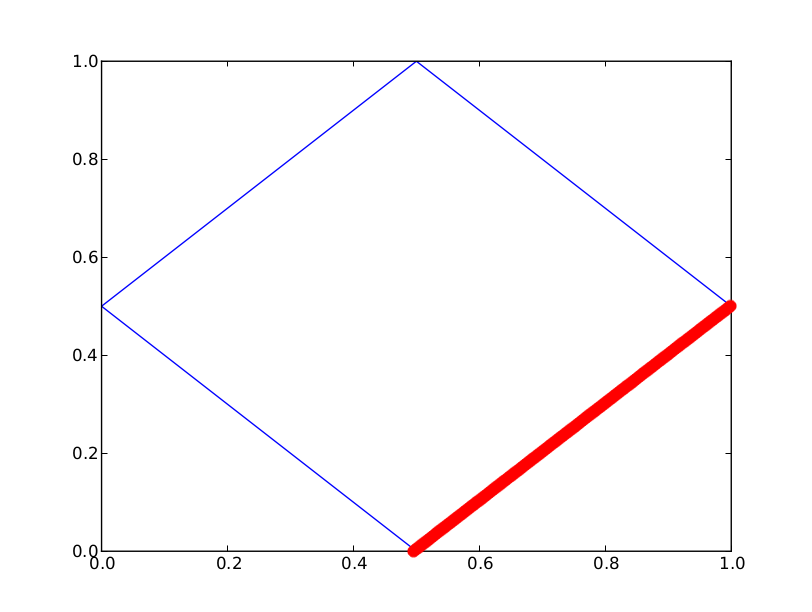
\includegraphics[width=2.1in]{tiling_real_step_3.png}
      \end{figure}
    \end{column}
    \begin{column}{0.45\textwidth}
      \begin{figure}
        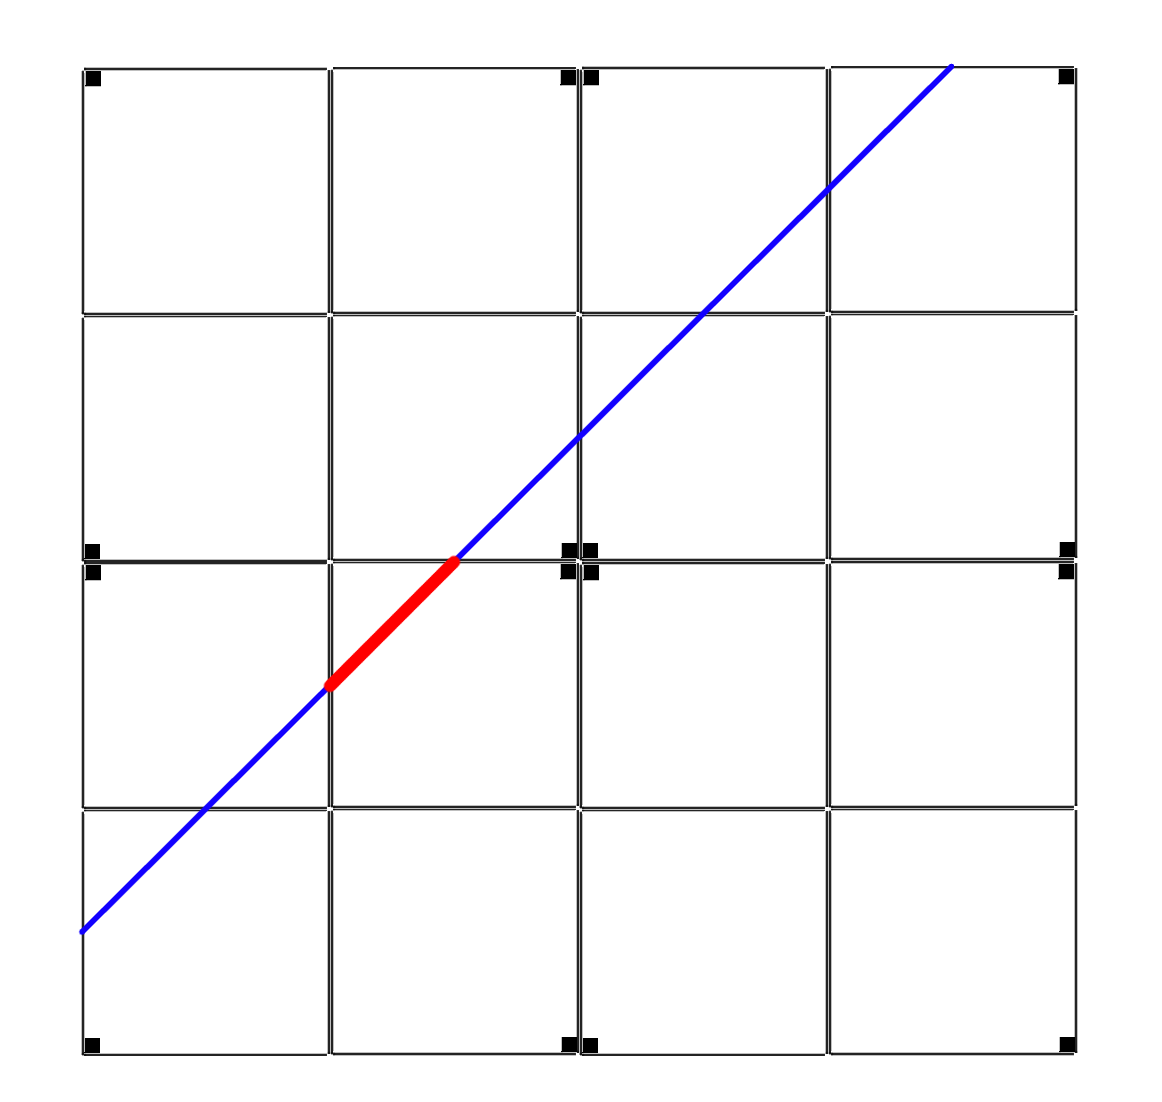
\includegraphics[width=1.7in]{tiling_tiled_step_3.png}
      \end{figure}
    \end{column}
  \end{columns}
}

\frame{
  \frametitle{Representing Collision Strings}

  \begin{example}
    Tiling of $\vec{x}_0 = (0, 0.5)$ and $\vec{v} = (0.25, 0.25)$.
  \end{example}

  \begin{columns}
    \begin{column}{0.45\textwidth}
      \begin{figure}
        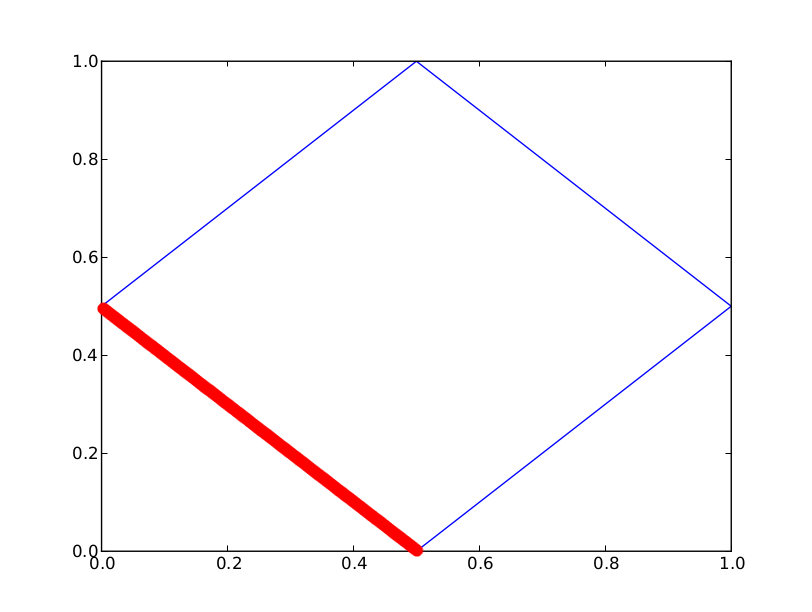
\includegraphics[width=2.1in]{tiling_real_step_4.png}
      \end{figure}
    \end{column}
    \begin{column}{0.45\textwidth}
      \begin{figure}
        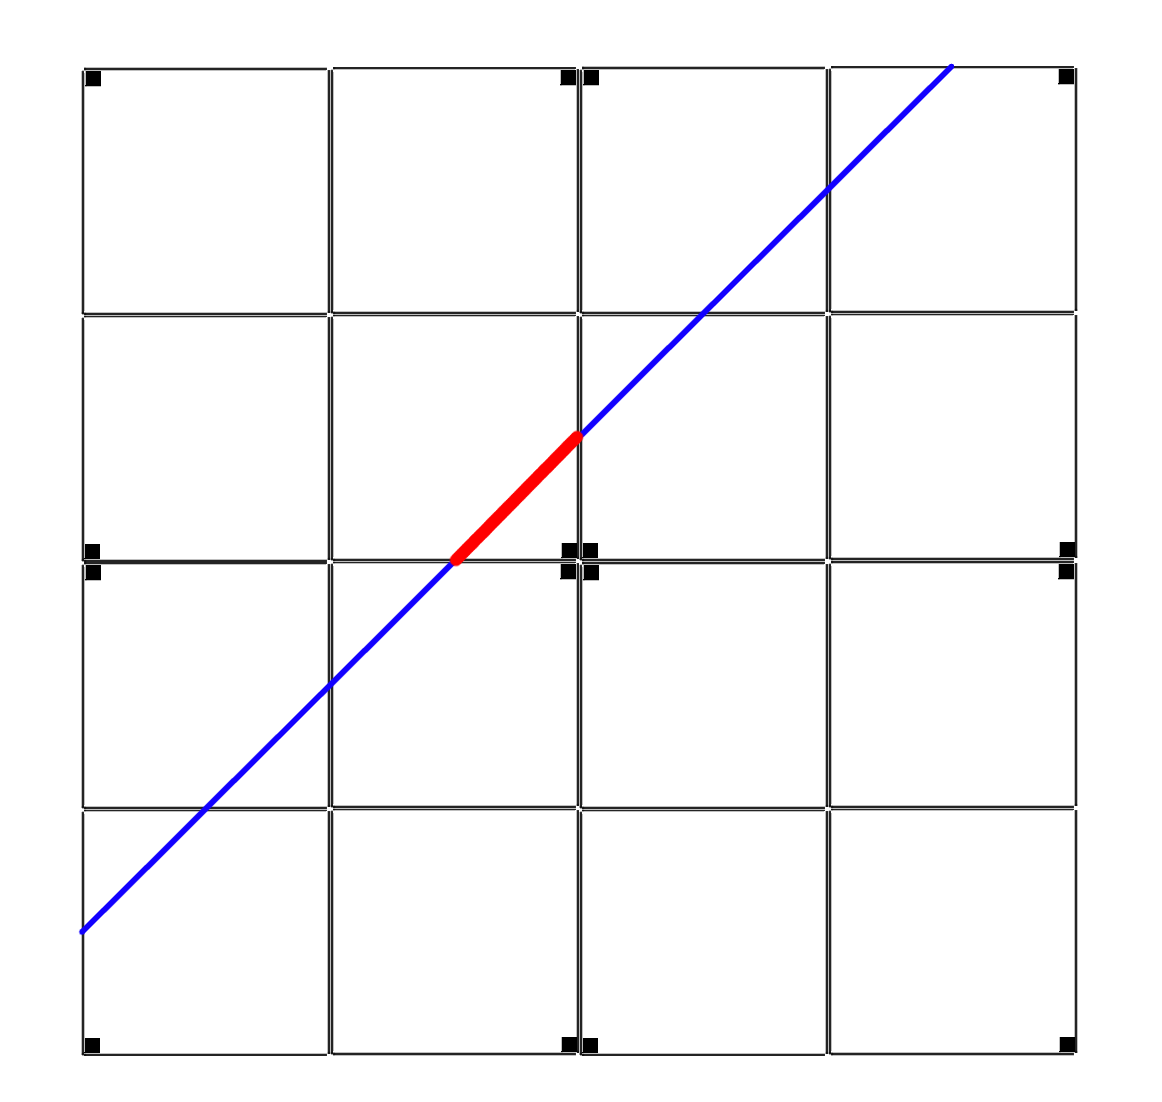
\includegraphics[width=1.7in]{tiling_tiled_step_4.png}
      \end{figure}
    \end{column}
  \end{columns}
}

\frame{
  \frametitle{Representing Collision Strings}

  \begin{example}
    Tiling of $\vec{x}_0 = (0, 0.5)$ and $\vec{v} = (0.25, 0.25)$.
  \end{example}

  \begin{columns}
    \begin{column}{0.45\textwidth}
      \begin{figure}
        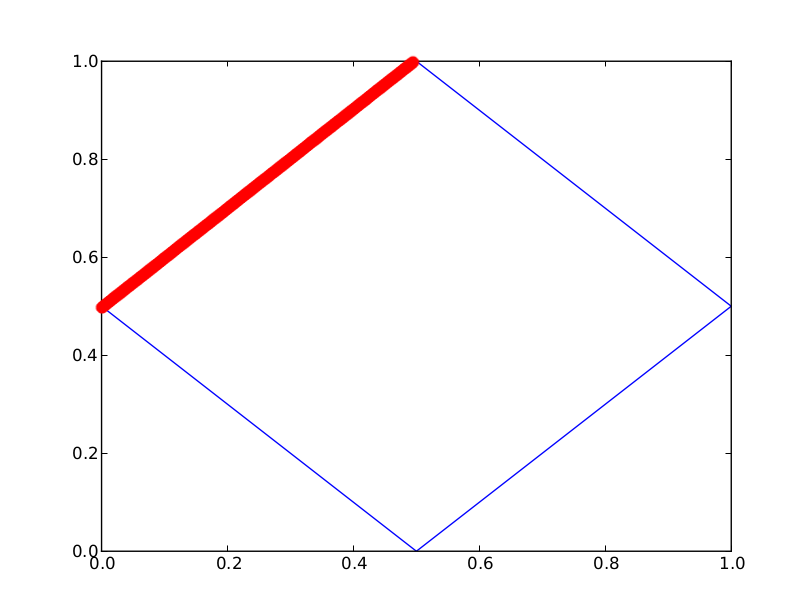
\includegraphics[width=2.1in]{tiling_real_step_1.png}
      \end{figure}
    \end{column}
    \begin{column}{0.45\textwidth}
      \begin{figure}
        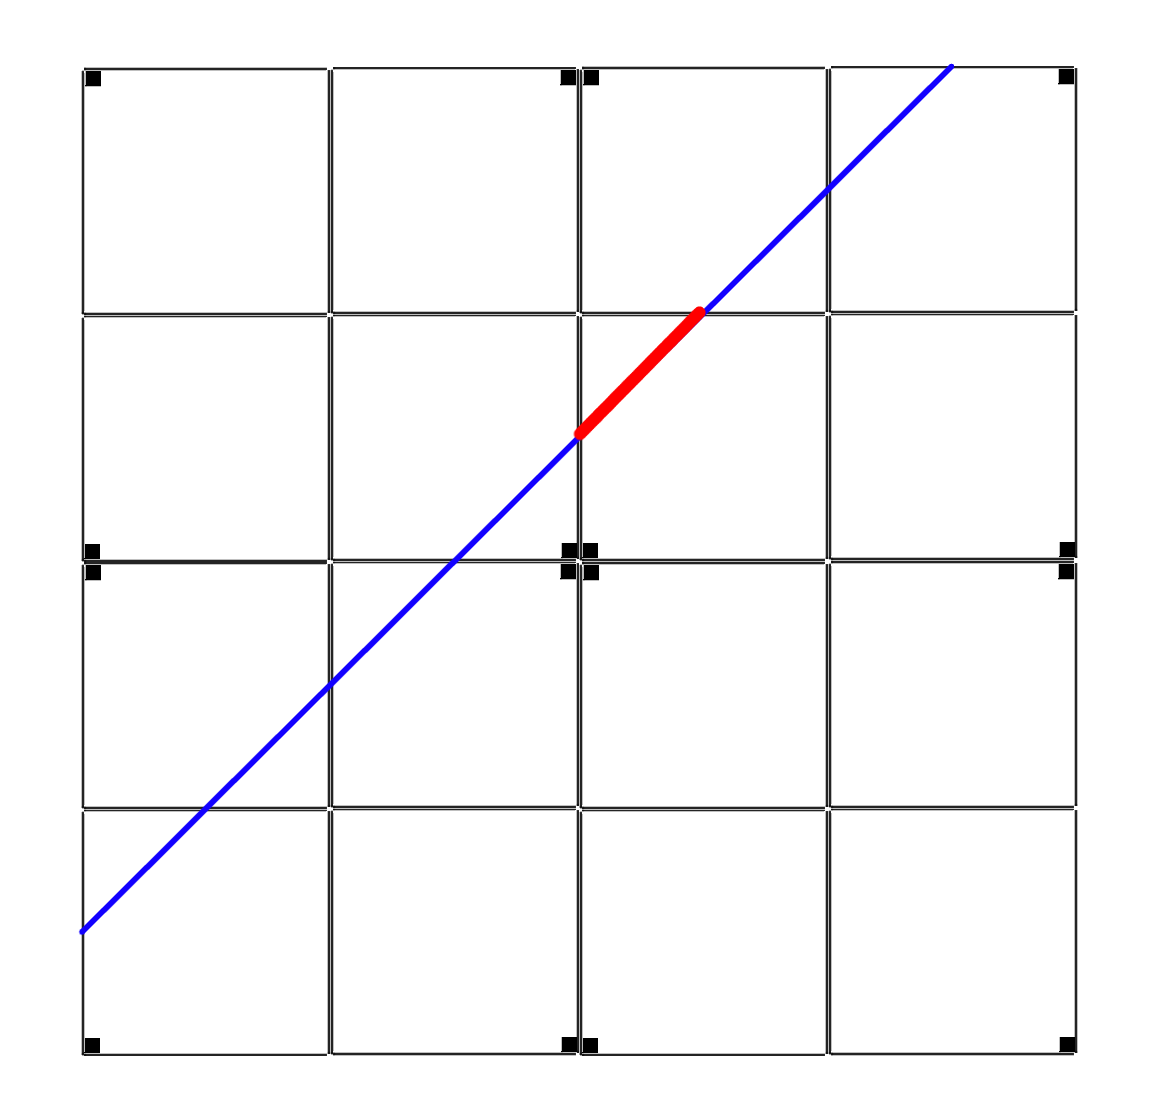
\includegraphics[width=1.7in]{tiling_tiled_step_5.png}
      \end{figure}
    \end{column}
  \end{columns}
}

\frame{
  \frametitle{Representing Collision Strings}

  \begin{example}
    Tiling of $\vec{x}_0 = (0, 0.5)$ and $\vec{v} = (0.25, 0.25)$.
  \end{example}

  \begin{columns}
    \begin{column}{0.45\textwidth}
      \begin{figure}
        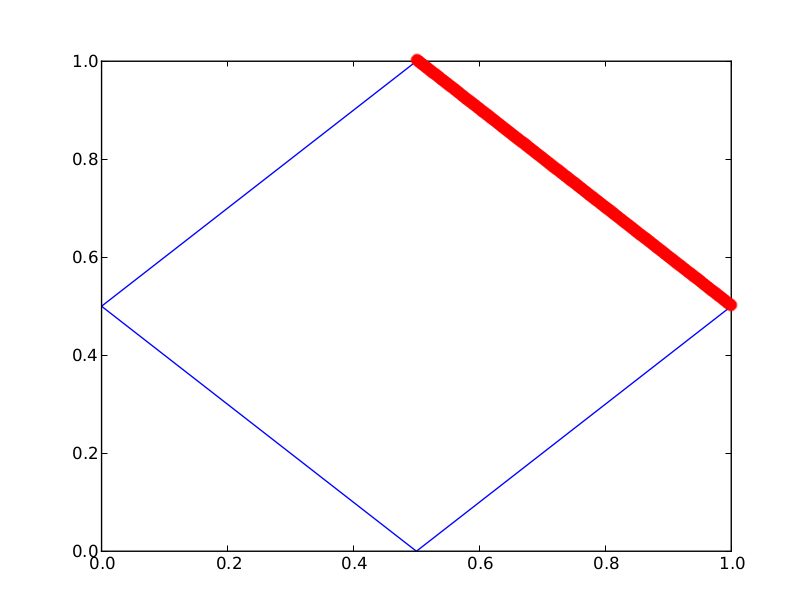
\includegraphics[width=2.1in]{tiling_real_step_2.png}
      \end{figure}
    \end{column}
    \begin{column}{0.45\textwidth}
      \begin{figure}
        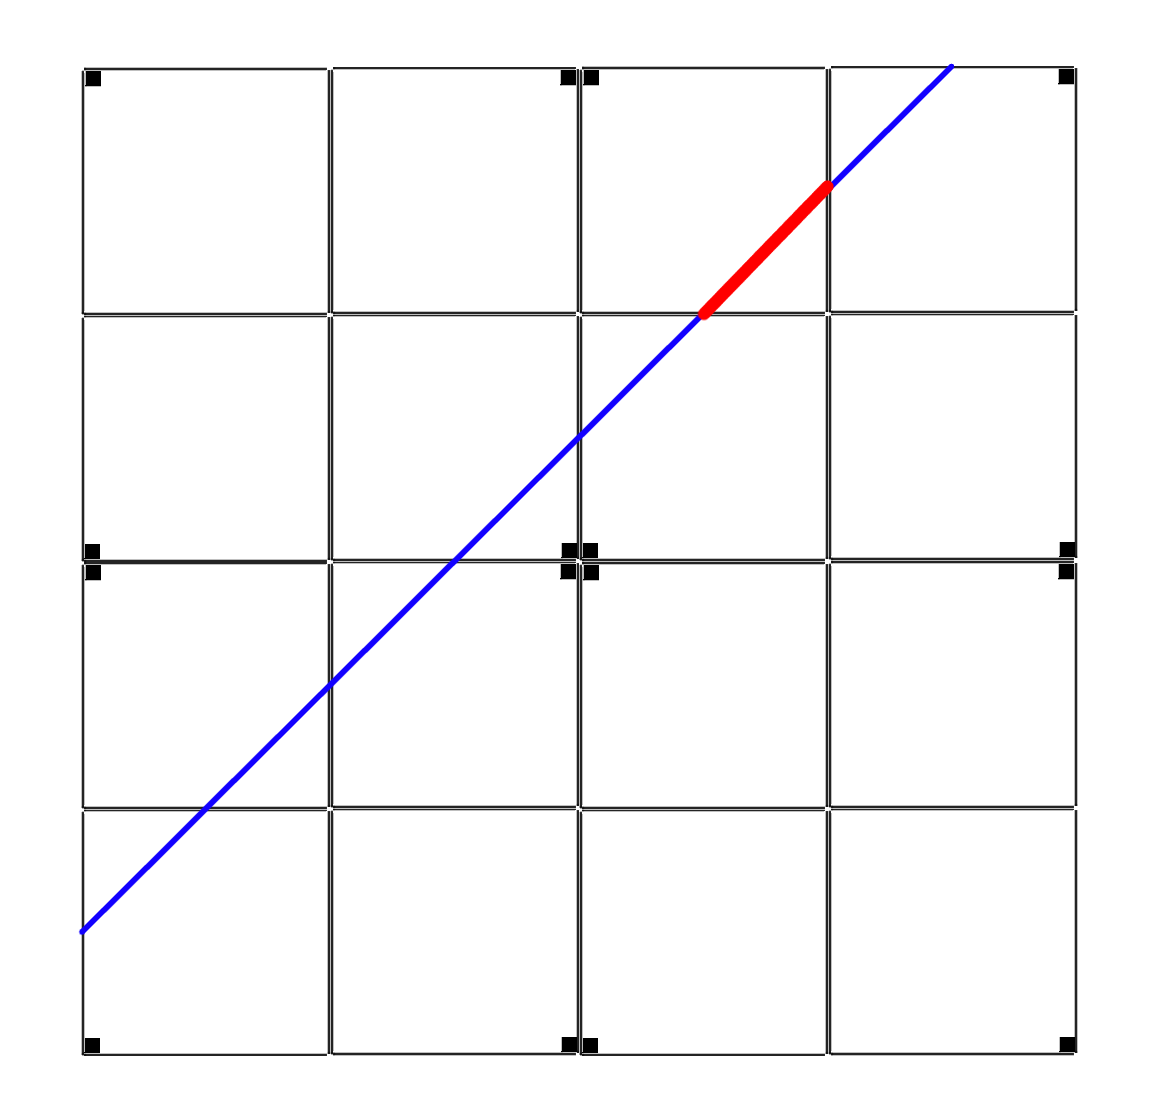
\includegraphics[width=1.7in]{tiling_tiled_step_6.png}
      \end{figure}
    \end{column}
  \end{columns}
}

\frame{
  \frametitle{Representing Collision Strings}

  \begin{example}
    Tiling of $\vec{x}_0 = (0, 0.5)$ and $\vec{v} = (0.25, 0.25)$.
  \end{example}

  \begin{columns}
    \begin{column}{0.45\textwidth}
      \begin{figure}
        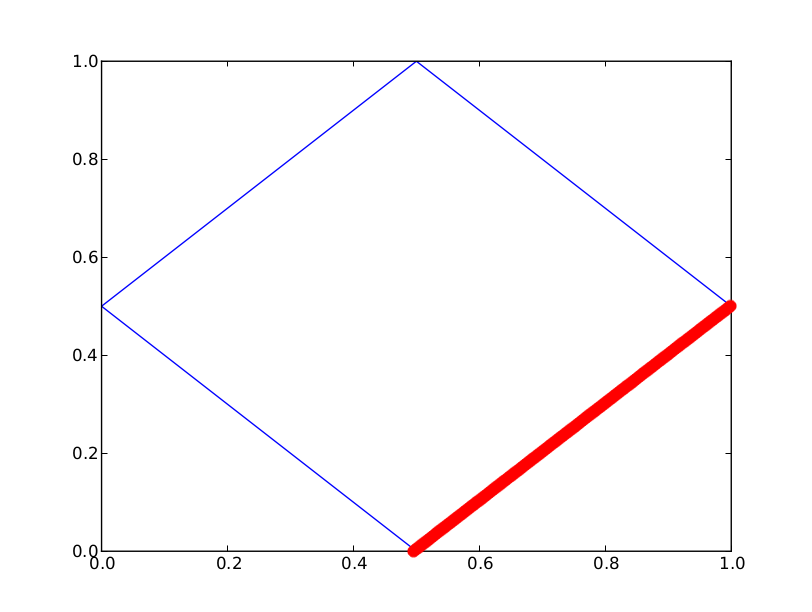
\includegraphics[width=2.1in]{tiling_real_step_3.png}
      \end{figure}
    \end{column}
    \begin{column}{0.45\textwidth}
      \begin{figure}
        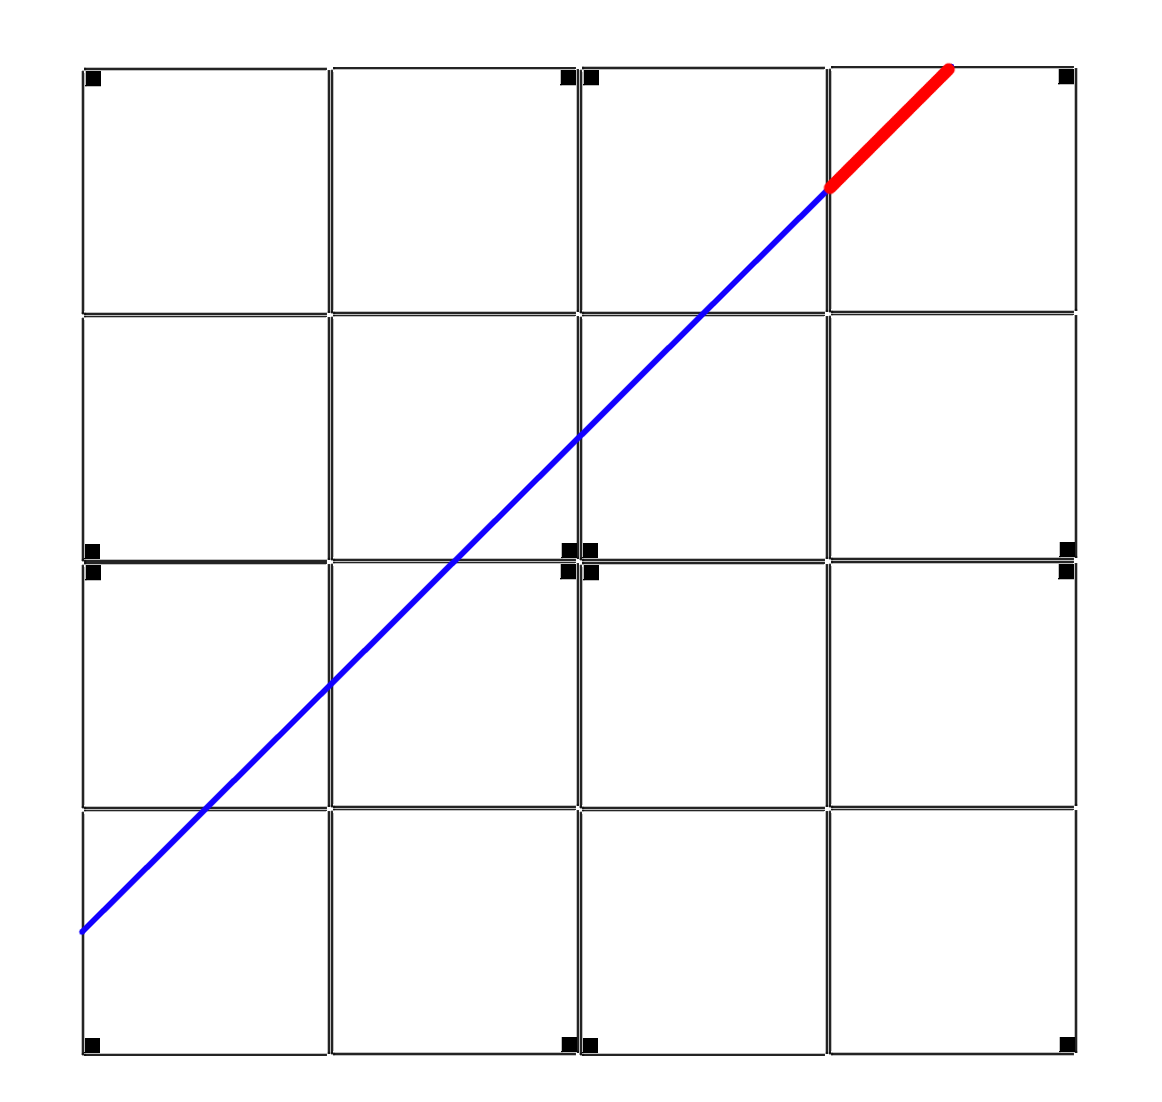
\includegraphics[width=1.7in]{tiling_tiled_step_7.png}
      \end{figure}
    \end{column}
  \end{columns}
}

\subsection{1-dimensional Problem}

\frame{
  \frametitle{Sequence Characterization}

  \begin{multline*}
    \begin{array}{cccccccccc}
      \underbrace{aaa} & b & \underbrace{aa} & b & \underbrace{aa} & b & \underbrace{aaa} & b & \underbrace{aa} & b \\
      3 && 2 && 2 && 3 && 2 &
    \end{array}\\
    \begin{array}{cccccccc}
      \underbrace{aa} & b & \underbrace{aaa} & b & \underbrace{aa} & b & \underbrace{aaa} & \dots \\
      2 && 3 && 2 && 3 & \dots
    \end{array}
  \end{multline*}
}

\frame{
  \frametitle{Sequence Characterization}

  \begin{gather*}
    \begin{array}{cccccccc}
      3 & \underbrace{22} & 3 & \underbrace{22} & 3 & \underbrace{2} & 3 & \dots\\ 
      & 2 && 2 && 1 & \dots
    \end{array}
  \end{gather*}
}
